\documentclass[
    11pt,
    a4paper,
    sfdefaults=false,
    toc=chapterentrywithdots,
    twoside,openright,
    titlepage,
    parskip=half,
    headings=normal,  % reduces heading size
    listof=totoc,
    bibliography=totoc,
    index=totoc,
    captions=tableheading,  % caption below table
    chapterprefix,
    listof=flat,
    final
]{scrbook}


% details about your thesis
\newcommand{\titel}{Gefahren im Metaverse: Social Engineering als Grundlage für Angriffe im Metaverse}
\newcommand{\artderarbeit}{Bachelorarbeit}  % {Bachelorarbeit,Masterarbeit}
\newcommand{\autor}{Andre Schindler}
\newcommand{\studiengang}{Wirtschaftsinformatik}  % {Informatik,Wirtschaftsinformatik,Medieninformatik}
\newcommand{\matrikelnr}{327\,2457}
\newcommand{\erstgutachter}{Prof.\,Dr.~Ronald Petrlic}
\newcommand{\zweitgutachter}{Prof.\,Dr.~Peter Rausch}
\newcommand{\betreuer}{M.Sc.\,~Martina Schmidt}
\newcommand{\unternehmen}{Musterfirma GmbH}
\newcommand{\logo}{figures/TH-Nuernberg-RGB.png}
\newcommand{\keywords}{hot, fuzz}
 

% custom head and foot
\usepackage[automark]{scrlayer-scrpage}
\pagestyle{scrheadings}
\ihead{\headmark}
\chead{}
\ohead{\pagemark}
\renewcommand*\chaptermarkformat{\chapappifchapterprefix{\ }% 
  \thechapter.\enskip}

\RedeclareSectionCommand[tocindent=10pt]{section}
\RedeclareSectionCommand[tocindent=18pt]{subsection}
%\RedeclareSectionCommand[tocnumwidth=0pt]{chapter}

\usepackage{scrhack}

% other packages
\usepackage[utf8]{inputenc}
\usepackage[T1]{fontenc}
\usepackage{lmodern,relsize,textcomp,csquotes}
\usepackage{amsmath,amsfonts}
\usepackage[ngerman]{babel}  % flip for German thesis
\usepackage[final]{graphicx}
\usepackage{setspace,geometry,xcolor}
\usepackage{makeidx}
\usepackage{paralist,ifthen,todonotes}
\usepackage{url}
\usepackage[toc, style=alttree]{glossaries}
\usepackage{pdfpages}

% table setup
\usepackage{longtable}
\usepackage{array}
\usepackage{ragged2e}
\usepackage{lscape}

% pdf hyperref
\usepackage[
    bookmarks=true,
    bookmarksopen=true,
    bookmarksnumbered=true,
    bookmarksopenlevel=1,
    pdftitle={\titel},
    pdfauthor={\autor},
    pdfcreator={\autor},
    pdfsubject={\titel},
    pdfkeywords={\keywords},
    pdfpagelabels=true,
    colorlinks=true,
    linkcolor=red,
    urlcolor=magenta,
    anchorcolor=black,
    citecolor=cyan,
    filecolor=magenta,
    menucolor=red,
    plainpages=false,
    hypertexnames=true,
    linktocpage=true,
]{hyperref}

% configure your listings style
\usepackage{listings}
\lstset{
	tabsize=3,
	extendedchars=true,
	frame=single,
	showstringspaces=true,
	numbers=left,
	numberstyle=\small,
	breakautoindent=true
}

% page setup
% \setlength{\topskip}{\ht\strutbox}
\geometry{paper=a4paper,left=2.5cm,top=3.0cm,bindingoffset=.8cm}
\onehalfspacing
\frenchspacing
\clubpenalty = 10000
\widowpenalty = 10000 
\displaywidowpenalty = 10000

% some commands
\newcommand{\ua}{\mbox{u.\,a.\ }}
\newcommand{\zB}{\mbox{z.\,B.\ }}
\newcommand{\dahe}{\mbox{d.\,h.,\ }}
\newcommand{\bzw}{\mbox{bzw.\ }}
\newcommand{\bzgl}{\mbox{bzgl.\ }}
\newcommand{\eg}{\mbox{e.\,g.\ }}
\newcommand{\ie}{\mbox{i.\,e.\ }}
\newcommand{\wrt}{\mbox{w.\,r.\,t.\ }}
\newcommand{\etal}{\mbox{\emph{et\,al.\ }}}


% TODO remove if not needed...
\usepackage{blindtext}

% load glossary entries
\makenoidxglossaries
\loadglsentries{glossary}
\glssetwidest{Immersion} %Glossar spaltenbreite festlegen

\begin{document}

\setcounter{secnumdepth}{3}  % numerate subsections
\setcounter{tocdepth}{2}  % ...but don't include them in toc

\frontmatter
\include{cover}\cleardoublepage

% download the following form and complete it (hit save in your editor)
% https://intern.ohmportal.de/fileadmin/Gelenkte_Doks/Abt/SZS/SB/SB_0050_FO_Pruefungsrechtliche_Erklaerung_und_Erklaerung_zur_Veroeffentlichung_der_Abschlussarbeit_public.pdf
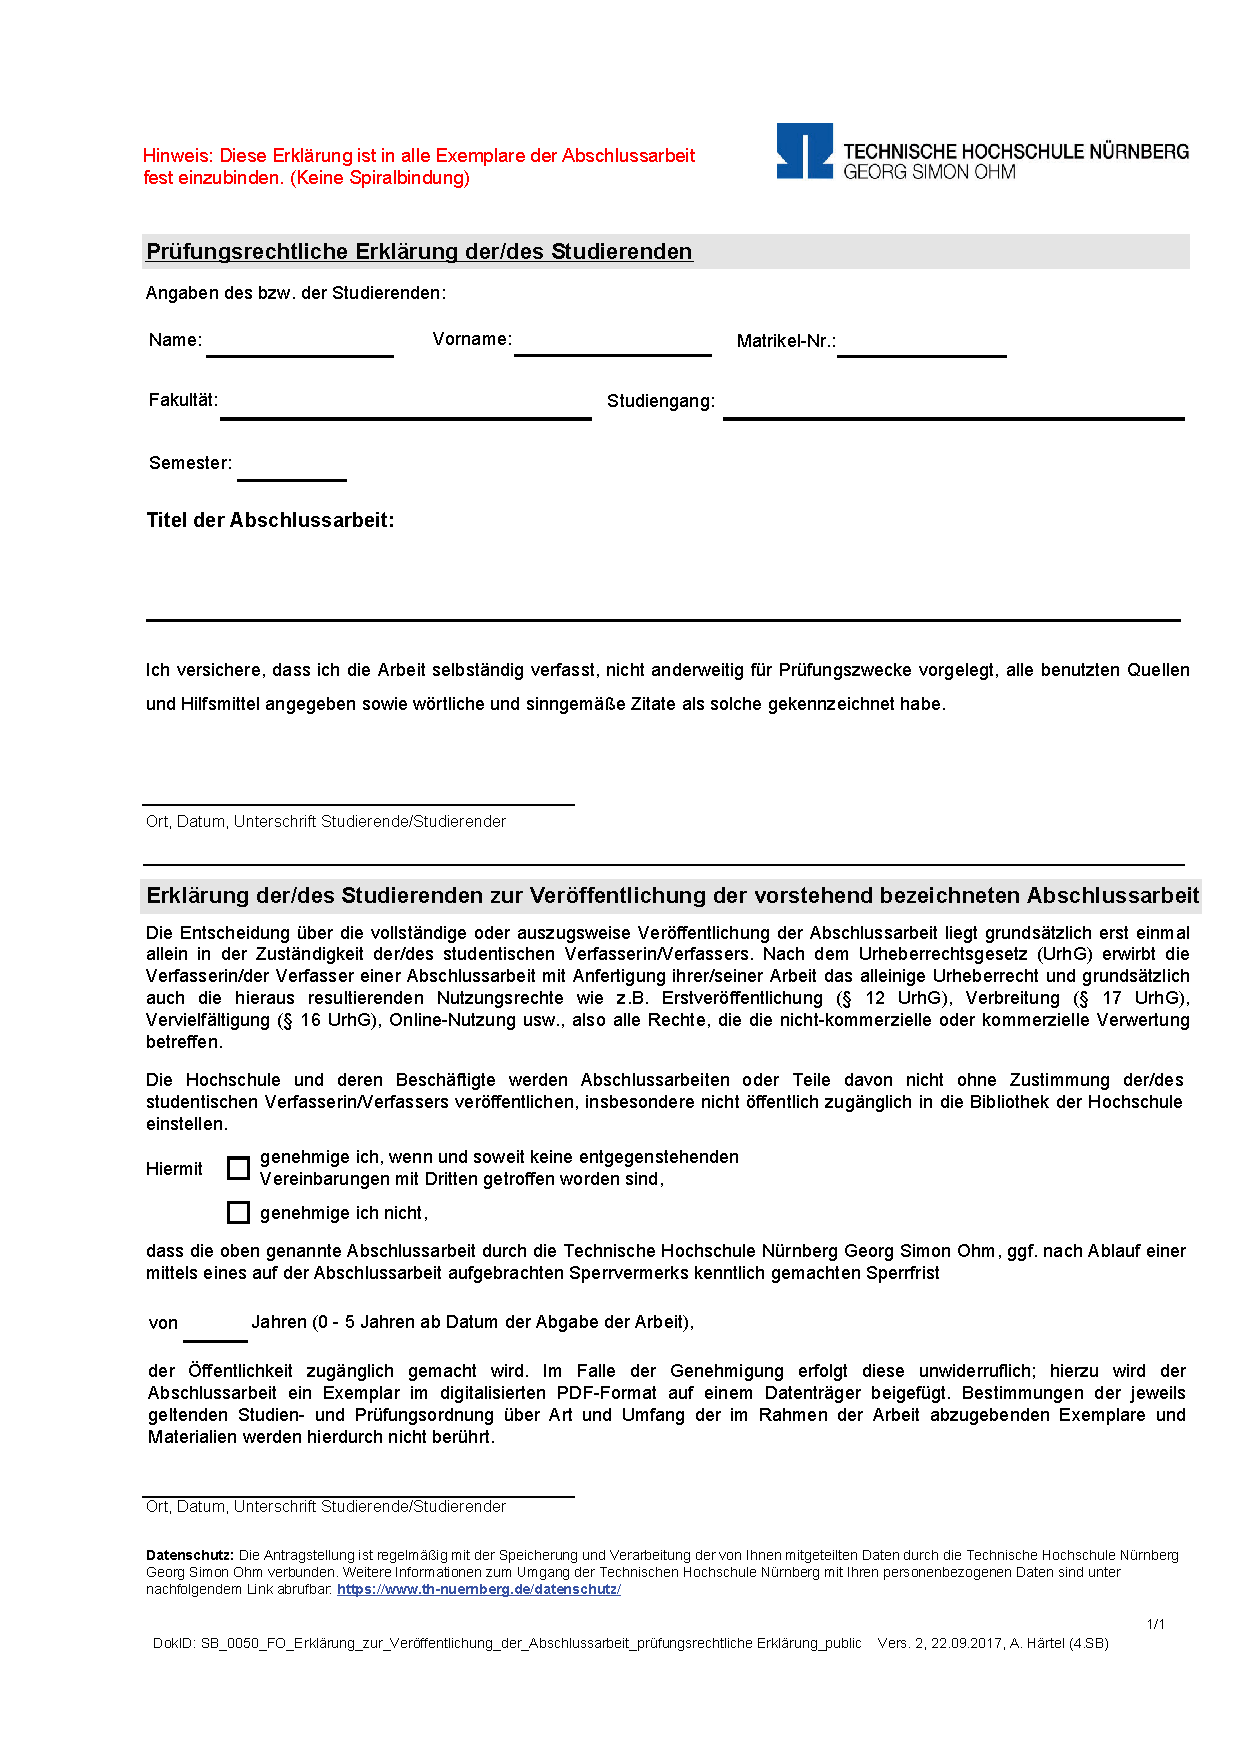
\includepdf{SB_0050_FO_Pruefungsrechtliche_Erklaerung_und_Erklaerung_zur_Veroeffentlichung_der_Abschlussarbeit_public.pdf}\cleardoublepage

\chapter{Anleitungen und Tests}\label{ch:Anleitungen}

\section{Anleitungen}

\paragraph*{Glossar}

Glossar erstellen \url{https://www.lektorat-bachelorarbeit.de/glossar-erstellen/#:~:text=In%20einem%20Glossar%20sammelt%20man,die%20Erstellung%2C%20beantwortet%20dieser%20Text.} \\
It is possible to reference glossary entries as \gls{library} as an example.

\paragraph{Bilder einfügen}
nach paragraph muss was stehen bevor das bild kommt

\begin{figure}[!h]
    \centering
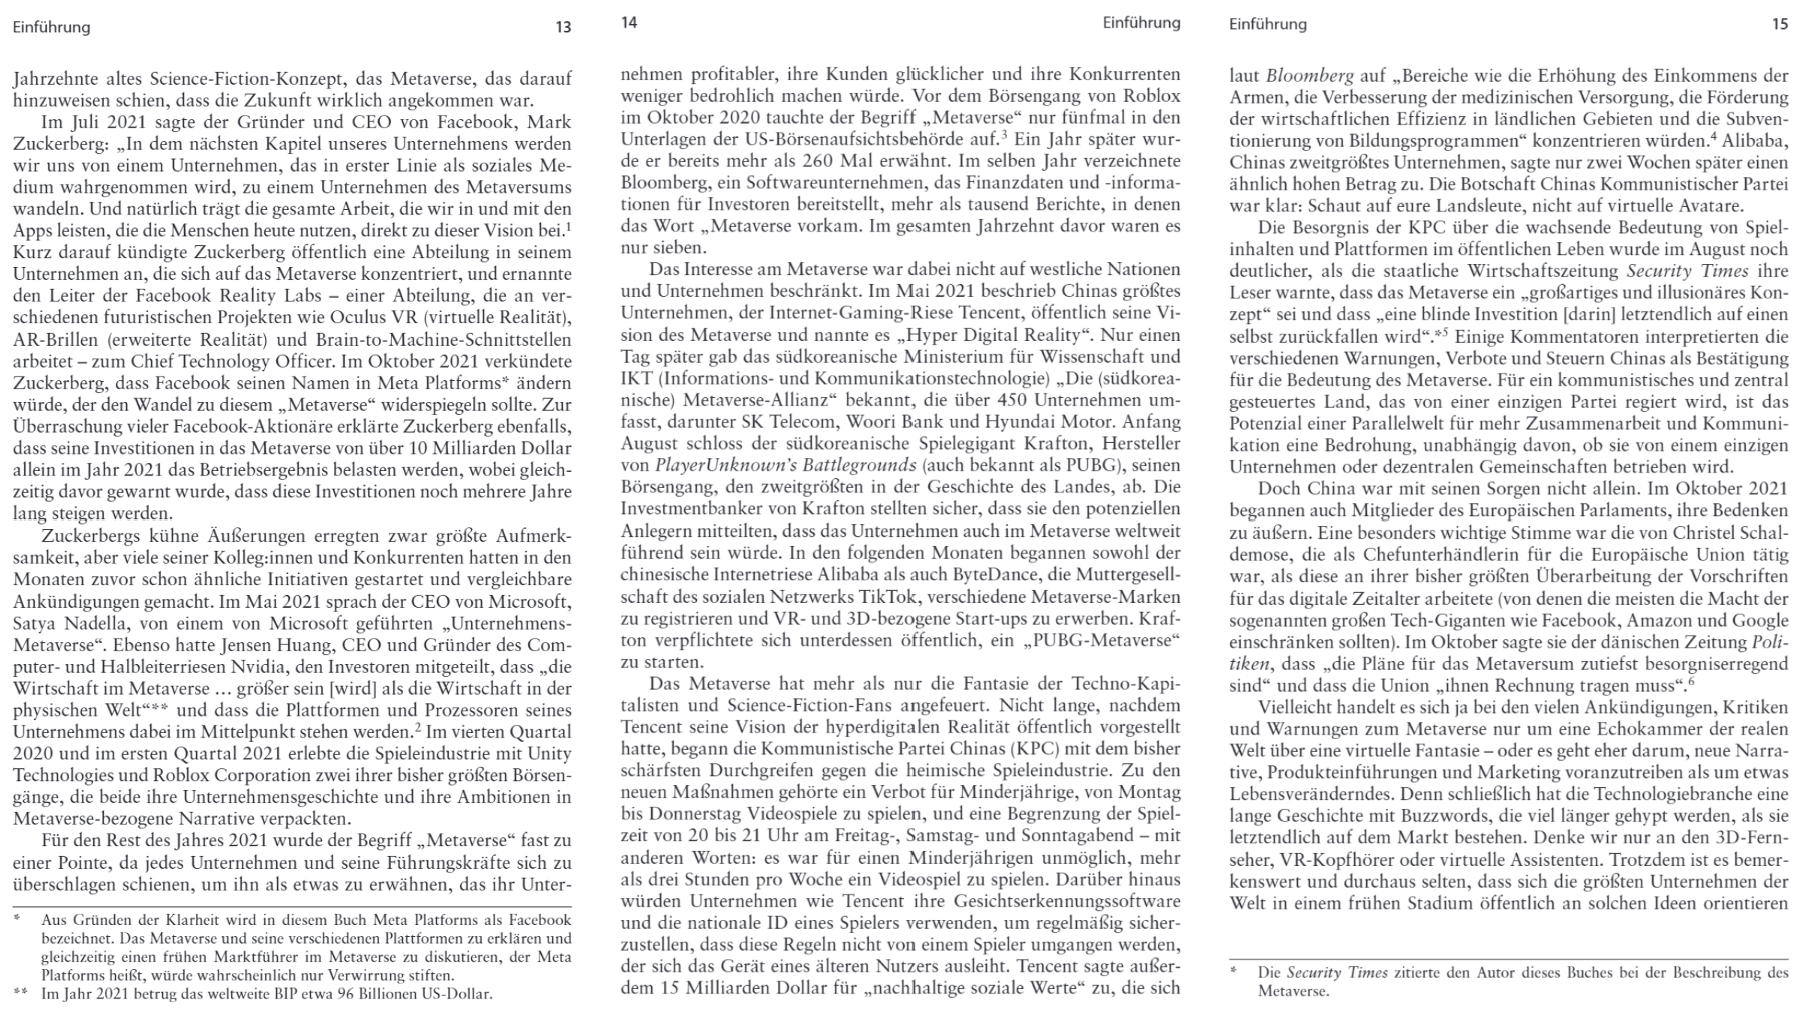
\includegraphics[width = 15cm]{figures/Das_Metaverse_uwearw13-15.png}
\caption{Das Metaverse und wie es alles revolutionieren wird}
\cite{Ball22}
\label{fig:testbild}
\end{figure}

%In this chapter, we're actually using some code!\\

%\begin{lstlisting}[language=Python,caption={This is an example of inline listing},captionpos=b]
%x = 1
%if x == 1:
%    # indented four spaces
%    print("x is 1.")

%\end{lstlisting}

%You can also include listings from a file directly:

%\lstinputlisting[language=Python,caption={This is an example of included listing},captionpos=b]{listings/example.py}


\section*{Tests}

Definitionen Metaverse \cite{Ball22}
\\Definitionen Metaverse \cite{Ball22a}
\\Definitionen Metaverse \cite{Drip22} \\
Seite 46 gegen wen Kämpfen wir \cite{Hypp22}\\
Psychologie hinter SocialEngeneering \cite{schu11}\\
\\

URL einfügen \url{https://ar5iv.labs.arxiv.org/html/2401.05569}


You can also write footnotes.\footnote{Footnotes will be positioned automatically.}

äüö


\thispagestyle{empty}
\section*{Kurzdarstellung}
\label{sec:kurzdarstellung}

\subsection{Was ist zu tun}
Kurze Zusammenfassung der Arbeit, höchstens halbe Seite.
Nenne die Zielsetzung, die Problemstellung und die Forschungsfragen. Wenn deiner Abschlussarbeit bestimmte Hypothesen zugrunde liegen, erwähne diese auch.
\\ \url{https://www.scribbr.de/aufbau-und-gliederung/abstract-schreiben/}


\subsection{Kurzdarstellung}
Das Ziel in der vorliegenden Arbeit ist es, zu klären, durch welche\dots


\cleardoublepage

\tableofcontents

\mainmatter
\chapter{Einleitung}\label{ch:Einleitung}

\paragraph*{TODO}
Diese Einleitung setzt den Ton für eine gründliche Analyse der Gefahren durch Social Engineering im Metaverse und skizziert den Aufbau sowie die Ziele der Arbeit. Sie betont sowohl die Aktualität als auch die Relevanz des Themas für ein breites Publikum einschließlich Akademikerinnen, Entwicklerinnen sowie Endnutzer*innen.

\subsection*{copy}

Die rasante Entwicklung digitaler Technologien hat in den letzten Jahren zu einem immer stärkeren Einzug virtueller Welten in unseren Alltag geführt. Das Konzept des Metaversums, einer immersiven und interaktiven virtuellen Realität, gewinnt zunehmend an Bedeutung und verspricht neue Möglichkeiten der Kommunikation, des Austauschs und der Unterhaltung. Doch mit dem Aufstieg des Metaversums gehen auch neue Gefahren einher, insbesondere im Hinblick auf die Manipulation und Täuschung von Nutzern durch Social Engineering.



Mit dem Aufkommen des Metaverse, einer konvergenten virtuellen Raumzeit, die durch die Verschmelzung von erweiterten (Augmented Reality) und virtuellen Realitäten (Virtual Reality) entsteht, eröffnen sich neue Dimensionen menschlicher Interaktion und digitaler Existenz. Diese immersive Plattform verspricht eine Revolution in der Art und Weise, wie wir kommunizieren, arbeiten, spielen und soziale Bindungen knüpfen. 

Das Metaverse, ein Konzept, das aus der Verschmelzung virtueller Realität, Augmented Reality und Internet entsteht, wird zunehmend als die nächste Entwicklungsstufe digitaler Interaktion betrachtet. Es verspricht eine umfassendere, immersivere Art der Online-Erfahrung, in der Nutzer nicht nur Inhalte konsumieren, sondern auch in einer dreidimensionalen Welt interagieren können.


Die digitale Revolution und die rasante Entwicklung virtueller Welten haben neue Räume für menschliche Interaktionen geschaffen. Insbesondere das Metaverse, eine kollektive virtuelle geteilte Raum, der durch die Konvergenz physisch persistenter virtueller Welten, einschließlich des Internets, entsteht, hat weitreichende Implikationen für soziale Dynamiken und Sicherheitsrisiken. Ein signifikantes Risiko in diesen virtuellen Umgebungen ist das des Social Engineering, bei dem menschliche Interaktionen ausgenutzt werden, um vertrauliche Informationen zu erhalten oder Benutzer zu unerwünschten Aktionen zu bewegen. Diese Bachelorarbeit untersucht Social Engineering als Grundlage für Angriffe im Metaverse, indem sie psychologische Prinzipien, Methoden, spezifische Risiken im Metaverse und Abwehrstrategien beleuchtet.


1. Einleitung
Das Metaverse, eine konvergente virtuelle und physische Realität, hat in den letzten Jahren zunehmend an Bedeutung gewonnen. Mit Technologien wie Virtual Reality (VR), Augmented Reality (AR) und Blockchain entwickelt sich das Metaverse zu einer neuen digitalen Umgebung, in der soziale Interaktionen, Geschäftsaktivitäten und tägliche Aufgaben nahtlos miteinander verschmelzen. Parallel dazu stellt Social Engineering eine wachsende Bedrohung dar, da es die menschliche Schwachstelle in der digitalen Sicherheit ausnutzt. Diese Bachelorarbeit untersucht die Auswirkungen von Social Engineering im Metaverse und bietet eine umfassende Analyse der daraus resultierenden persönlichen, sozialen und wirtschaftlichen Folgen.


\section{Problemstellung}
\subsection*{copy}

Social Engineering, als eine Form der sozialen Manipulation, zielt darauf ab, das Vertrauen von Menschen zu gewinnen und sie dazu zu bringen, sensible Informationen preiszugeben oder unerwünschte Handlungen auszuführen. Im Kontext des Metaversums können Social Engineering-Angriffe schwerwiegende Folgen haben, da die Grenzen zwischen realer und virtueller Welt verschwimmen und Nutzer sich in einer Umgebung bewegen, die oft als sicher wahrgenommen wird.


Mit den unzähligen Möglichkeiten des Metaverse gehen auch Risiken einher; insbesondere die Gefahren durch Social Engineering stellen eine ernstzunehmende Bedrohung dar.
Social Engineering bezeichnet die Kunst der Manipulation von Menschen, um sie dazu zu bringen, vertrauliche Informationen preiszugeben oder bestimmte Handlungen auszuführen, die normalerweise gegen ihre eigenen Interessen oder Sicherheitsprotokolle verstoßen würden. Im Kontext des Metaverse gewinnt diese Form der Bedrohung aufgrund der tiefgreifenden Vernetzung und der oft noch unausgereiften Sicherheitsmechanismen an Brisanz.


Bedeutung von Social Engineering
Social Engineering spielt in der Cybersecurity eine zentrale Rolle, da es sich auf die Ausnutzung menschlicher Fehler konzentriert, um unbefugten Zugang zu Informationen oder Systemen zu erlangen. Im Kontext des Metaverse gewinnt Social Engineering aufgrund der tiefen Immersion und des verstärkten sozialen Engagements eine neue Dimension.

Social Engineering nutzt grundlegende menschliche Verhaltensweisen und psychologische Manipulation, um Sicherheitsmechanismen zu umgehen. Im Kontext des Internets und digitaler Umgebungen wurden verschiedene Angriffsmethoden identifiziert, die von Phishing bis hin zu komplexen Betrugsschemata reichen. \url{https://ar5iv.labs.arxiv.org/html/2203.08302} Die Übertragung dieser Methoden auf das Metaverse ist durch die immersive und sozial vernetzte Natur dieser Welten besonders besorgniserregend.

Das Metaverse verstärkt die Wirkung von Social Engineering durch seine Fähigkeit, tiefe soziale Verbindungen und Interaktionen zu ermöglichen, die über traditionelle Online-Plattformen hinausgehen. Es bietet eine reichhaltige Umgebung für Täter, um vertrauenswürdige Identitäten zu simulieren oder manipulative Szenarien zu erstellen, die schwer zu erkennen sind. \url{https://ar5iv.labs.arxiv.org/html/2203.04813} \url{https://ar5iv.labs.arxiv.org/html/2401.05569} Zudem erhöht die Anonymität und Skalierbarkeit von Interaktionen im Metaverse die Herausforderungen bei der Identifizierung und Verhinderung von Social Engineering-Angriffen.

Die Erkennung und Abwehr von Social Engineering im Metaverse erfordert innovative Ansätze, die sowohl technologische als auch soziale Strategien umfassen. Maschinelles Lernen und künstliche Intelligenz bieten Potenziale für die Erkennung von Angriffsmustern und ungewöhnlichen Verhaltensweisen. \url{https://arxiv.org/abs/2203.07933} \url{https://ar5iv.labs.arxiv.org/html/2401.05569} Gleichzeitig sind Bildung und Bewusstsein über Social Engineering-Methoden entscheidend, um Nutzer im Metaverse zu befähigen, potenzielle Bedrohungen zu erkennen und sich davor zu schützen.


1.1 Problemstellung
Mit der rasanten Entwicklung des Metaverse entstehen neue Formen sozialer Interaktionen und Geschäftsmodelle. Diese virtuelle Welt bietet immense Möglichkeiten, birgt jedoch auch erhebliche Risiken. Social Engineering, die Kunst der zwischenmenschlichen Manipulation, nutzt das Vertrauen und die Naivität von Nutzern aus, um sensible Informationen zu erlangen oder schädliche Handlungen zu provozieren. Im Metaverse, wo die Grenzen zwischen virtuellen und realen Identitäten verschwimmen, sind die potenziellen Auswirkungen solcher Angriffe noch gravierender. Nutzer können finanziell geschädigt werden, ihr digitales Vertrauen verlieren und emotional belastet werden. Unternehmen stehen vor Herausforderungen, ihre digitalen Vermögenswerte zu schützen und das Vertrauen ihrer Kunden zu erhalten. Trotz der zunehmenden Relevanz dieses Themas gibt es bisher nur begrenzte Forschung zu den spezifischen Auswirkungen von Social Engineering im Metaverse.

Beispielhafte Formulierung für die Problemstellung:
Das Metaverse revolutioniert die Art und Weise, wie Menschen interagieren, Geschäfte tätigen und sich in digitalen Umgebungen bewegen. Gleichzeitig eröffnet es neue Angriffspunkte für Social Engineering. Angreifer nutzen die immersive Natur des Metaverse, um Nutzer zu täuschen und auszunutzen. Dies kann schwerwiegende persönliche und wirtschaftliche Schäden verursachen. Trotz der wachsenden Bedeutung des Metaverse ist wenig darüber bekannt, wie Social Engineering in dieser neuen digitalen Umgebung funktioniert und welche spezifischen Risiken damit verbunden sind.


\section{Zielsetzung der Arbeit}
\subsection*{copy}


Das Ziel dieser Bachelorarbeit ist es, die Gefahren im Metaverse durch Social Engineering genauer zu untersuchen und Maßnahmen zur Prävention und Abwehr solcher Angriffe zu identifizieren. Dazu werden zunächst die theoretischen Grundlagen von Metaverse und Social Engineering erläutert, bevor konkrete Risiken und Angriffsszenarien im Metaverse analysiert werden. Anhand von Fallbeispielen aus der Praxis sollen die Auswirkungen erfolgreicher Social Engineering-Angriffe verdeutlicht werden.


Durch die Erarbeitung präventiver Maßnahmen sowie die Diskussion aktueller Herausforderungen und Zukunftsperspektiven im Bereich des Metaversums soll ein Beitrag zur Sensibilisierung für die Gefahren von Social Engineering geleistet werden. Diese Arbeit trägt somit dazu bei, das Bewusstsein für Sicherheitsaspekte im digitalen Raum zu schärfen und einen Beitrag zur Gestaltung einer vertrauenswürdigen virtuellen Umgebung zu leisten.

Die Bachelorarbeit verfolgt das Ziel, die Komplexität und Vielschichtigkeit der Gefahren im Metaverse durch Social Engineering aufzuzeigen und Lösungsansätze für eine sichere Nutzung virtueller Welten zu entwickeln. Dabei werden sowohl technische als auch soziale Aspekte berücksichtigt, um ein ganzheitliches Verständnis der Thematik zu ermöglichen.


Im Rahmen dieser Arbeit werden verschiedene Methoden der Datenerhebung und Analyse angewendet, um fundierte Erkenntnisse zu gewinnen und die Forschungsfragen adäquat zu beantworten. Durch die Analyse von Fallstudien und Praxisbeispielen sollen konkrete Einblicke in die Realität von Social Engineering-Angriffen im Metaverse gegeben werden.


Die vorliegende Bachelorarbeit leistet einen Beitrag zur aktuellen Diskussion über Sicherheitsrisiken im digitalen Raum und sensibilisiert für die potenziellen Gefahren, denen Nutzer im Metaverse ausgesetzt sind. Die Ergebnisse dieser Arbeit sollen dazu beitragen, das Bewusstsein für die Bedeutung von Sicherheitsmaßnahmen im virtuellen Raum zu stärken und einen Beitrag zur Schaffung einer vertrauenswürdigen und sicheren Umgebung im Metaverse zu leisten.

In den folgenden Kapiteln werden zunächst die theoretischen Grundlagen von Metaverse und Social Engineering erläutert, gefolgt von einer detaillierten Analyse der Gefahren im Metaverse durch Social Engineering. Anhand von praxisnahen Beispielen werden die Auswirkungen solcher Angriffe verdeutlicht und präventive Maßnahmen zur Abwehr von Social Engineering-Angriffen diskutiert. Abschließend erfolgt eine Zusammenfassung der wichtigsten Erkenntnisse sowie ein Ausblick auf zukünftige Entwicklungen in diesem Bereich.


Die vorliegende Arbeit trägt dazu bei, das Bewusstsein für die Gefahren von Social Engineering im Metaverse zu schärfen und liefert wichtige Impulse für die Weiterentwicklung von Sicherheitskonzepten in virtuellen Welten.


Diese Bachelorarbeit zielt darauf ab, die spezifischen Gefahren zu identifizieren und zu analysieren, die Social Engineering im Metaverse mit sich bringt. Dabei wird untersucht, wie Angreifer psychologische Tricks und Täuschungstechniken nutzen können, um Nutzer in dieser neuen digitalen Umgebung auszunutzen. Die Arbeit beleuchtet sowohl theoretische Grundlagen als auch praktische Beispiele und strebt danach, effektive Gegenmaßnahmen und Empfehlungen für Nutzer sowie Entwickler des Metaverse zu entwickeln.
Um den Rahmen dieser Untersuchung abzustecken, beginnt Kapitel 1 mit einer Einführung in das Konzept des Metaverse und dessen aktuelle technologische Landschaft. Kapitel 2 beschäftigt sich mit den Grundlagen des Social Engineering und dessen Evolution im digitalen Zeitalter. In Kapitel 3 werden dann spezielle Herausforderungen und Risiken des Social Engineering im Kontext des Metaverse dargelegt. Anschließend werden in Kapitel 4 Fallstudien präsentiert, welche reale Vorfälle von Social Engineering im Metaverse analysieren. Schließlich werden in Kapitel 5 Strategien zur Prävention und Sensibilisierung diskutiert, um Nutzer vor solchen Angriffen zu schützen.
Das Ziel dieser Arbeit ist es nicht nur, ein Bewusstsein für die potenziellen Gefahren zu schaffen, sondern auch dazu beizutragen, das Metaverse als einen sicheren Ort für zukünftige Generationen zu gestalten. In einer Welt, in der digitale Identitäten zunehmend an Bedeutung gewinnen und das Potenzial haben, unsere physische Realität zu beeinflussen, ist es von entscheidender Wichtigkeit, robuste Sicherheitskonzepte zu entwickeln und umzusetzen.


Zielsetzung und Forschungsfrage
Diese Arbeit zielt darauf ab, die Mechanismen und Risiken von Social Engineering-Angriffen im Metaverse zu untersuchen. Die zentrale Forschungsfrage lautet: "Wie nutzen Angreifer Social Engineering als Grundlage für Angriffe im Metaverse, und welche Maßnahmen können zur Prävention ergriffen werden?"


Diese Arbeit zielt darauf ab, ein umfassendes Verständnis von Social Engineering-Angriffen im Metaverse zu entwickeln und effektive Gegenmaßnahmen zu identifizieren. Durch die Analyse bestehender Forschung und Technologien sowie die Untersuchung spezifischer Fallstudien werden die einzigartigen Herausforderungen und Lösungsansätze für die Sicherheitsrisiken im Metaverse aufgezeigt und erörtert. Das Ziel ist, ein tieferes Verständnis für die Mechanismen von Social Engineering-Angriffen in diesen neuen digitalen Räumen zu schaffen und gleichzeitig praktikable Lösungen für ihre Prävention und Abwehr zu entwickeln.


1.2 Zielsetzung der Arbeit
Ziel dieser Bachelorarbeit ist es, die Auswirkungen von Social Engineering im Metaverse zu untersuchen. Es soll aufgezeigt werden, wie Social Engineering im Metaverse funktioniert, welche Techniken Angreifer anwenden und welche Folgen solche Angriffe haben können. Durch die Analyse von Fallstudien und die Betrachtung bestehender Sicherheitsmaßnahmen sollen Empfehlungen entwickelt werden, um die Nutzer im Metaverse besser zu schützen. Zudem wird die Arbeit darauf abzielen, das Bewusstsein für die potenziellen Gefahren von Social Engineering in dieser neuen digitalen Ära zu schärfen und Vorschläge für zukünftige Forschungsrichtungen zu geben.

Beispielhafte Formulierung für die Zielsetzung:
Diese Arbeit verfolgt das Ziel, die Mechanismen und Auswirkungen von Social Engineering im Metaverse zu analysieren. Es wird untersucht, wie Angreifer im Metaverse operieren, welche spezifischen Techniken sie anwenden und welche Auswirkungen dies auf Nutzer und Unternehmen hat. Durch die Untersuchung von Fallstudien und die Analyse bestehender Schutzmaßnahmen sollen Strategien entwickelt werden, um die Sicherheit im Metaverse zu erhöhen. Darüber hinaus soll die Arbeit das Bewusstsein für die Risiken von Social Engineering in virtuellen Welten stärken und Ansätze für zukünftige Forschungen aufzeigen.



\subsection*{Bilder}

\begin{figure}[h]
\centering
\includegraphics*{figures/Das_Metaverse_uwearw13-15.png}
\caption{Das Metaverse und wie es alles revolutionieren wird}
\label{fig:meine-grafik}
\cite{Ball22}
\end{figure}


Seit wann das Metaverse bekannt wurde \cite{Ball22a}
\chapter{Das Metaverse}\label{ch:Metaverse}

\section{Definition und Entwicklung} % oder Entwicklung
\section{Technologie}

\subsection{Virtuelle Realität}
\subsection{Augmented Realität}
\subsection{Digitale Zwillinge}
\subsection{Künstliche Intelligenz}
\subsection{LED und Hologramme}
\subsection{Kryptowährungen}
\subsection{Smart-Contracts}

\section{Beispiele}

\subsection{Meta}
\subsection{Sandbox}
\subsection{Roblox}
\subsection{Fortnite}
\subsection{Warframe}
\chapter{Social Engineering}\label{ch:SocialEngineering}

\section{Definition des Social Engineering}

>>Social Engineering benutzt Techniken der Beeinflussung und Überredungskunst zur Manipulation oder zur Vortäuschung falscher Tatsachen, über die sich ein Social Engineer eine gefälschte Identität aneignet. Damit kan der Social Engineer andere zu seinem Vorteil ausbeuten, um mit oder ohne Verwendung von technischen Hilfsmitteln an Informationen zu gelangen.<<\cite{mitn}

Was ist Social Engineering?
Beim Social Engineering werden menschliche Eigenschaften wie Hilfsbereitschaft, Vertrauen, Angst oder Respekt vor Autorität ausgenutzt, um Personen geschickt zu manipulieren. Cyber-Kriminelle verleiten das Opfer auf diese Weise beispielsweise dazu, vertrauliche Informationen preiszugeben, Sicherheitsfunktionen auszuhebeln, Überweisungen zu tätigen oder Schadsoftware auf dem privaten Gerät oder einem Computer im Firmennetzwerk zu installieren.\cite{bsi}

Akt der Manipulation einer Person, eine Handlung auszuführen, die vielleicht im besten Interesse der >>Zielperson<< liegt - oder auch nicht.\cite{Hadn1}

Arzte Psychologen und Therapeuthen nutzen beispielsweise oft Elemente des Social Engineering um ihre Patienten zu bestimmten Handlungen zu manipulieren. Trickbetrüger hingegen nutzen Elemente des Social Engineering um ihre Zielperson zu Aktivitäten zu bringen die zu einem Verlust führen \cite{Hadn1}

Social Engineering [...] nennt man zwischenmenschliche Beeinflussungen mit dem Ziel, bei Personen bestimmte Verhaltensweisen hervorzurufen, sie zum Beispiel zur Preisgabe von vertraulichen Informationen, zum Kauf eines Produktes oder zur Freigabe von Finanzmitteln zu bewegen.

Gleichzeitig steht Social Engineering für eine Praxis der politischen und gesellschaftlichen Steuerung bzw. Beeinflussung von Gesellschaften mittels Kommunikation und kann sowohl als positiv als auch als negativ wahrgenommene Ergebnisse erzielen. Die stark negative Begriffsvariante dominiert jedoch aktuell das Begriffsbild, gleichfalls gibt es alternative Definitionen für Social Engineering (Politikwissenschaft).\cite{test}

\section{Geschichte des Social Engineering}

\subsection*{copy}

\paragraph*{1}
Die Geschichte des Social Engineerings ist eng mit der Entwicklung menschlicher Kommunikation und Interaktion verbunden. Social Engineering bezeichnet in diesem Kontext die Kunst der Manipulation von Menschen, um sie dazu zu bringen, vertrauliche Informationen preiszugeben oder bestimmte Handlungen auszuführen. Diese Praktik kann für verschiedene Zwecke eingesetzt werden, von Spionage und Betrug bis hin zur Sicherheitsanalyse. Im Folgenden skizziere ich einige Schlüsselmomente und Entwicklungen in der Geschichte des Social Engineerings, die für deine Bachelorarbeit relevant sein könnten:

Frühe Geschichte und Kriegsführung: Bereits in antiken Geschichten und Kriegen spielte Social Engineering eine Rolle, etwa wenn Spione Informationen sammelten oder wenn durch List und Täuschung Kriege gewonnen wurden. Ein berühmtes Beispiel aus der griechischen Mythologie ist das Trojanische Pferd, das als Strategie betrachtet werden kann, den Feind durch Täuschung zu besiegen.

19. und frühes 20. Jahrhundert: Mit der Industrialisierung und der zunehmenden Komplexität der Gesellschaft nahmen auch Betrug und Täuschung zu. Berühmte Betrüger wie Victor Lustig, der angeblich den Eiffelturm "verkaufte", nutzten Social Engineering-Techniken, um ihre Betrügereien durchzuführen.

Zweiter Weltkrieg: Im Zweiten Weltkrieg wurde Social Engineering von verschiedenen Geheimdiensten eingesetzt, um Spionage zu betreiben und feindliche Operationen zu stören. Die Operation Fortitude, bei der die Alliierten die Deutschen über den tatsächlichen Ort der D-Day-Invasion täuschten, ist ein Beispiel für erfolgreiches Social Engineering.

Das Zeitalter der Informationstechnologie: Mit dem Aufkommen von Computern und dem Internet hat sich Social Engineering weiterentwickelt. Phishing-Angriffe, bei denen Betrüger versuchen, über gefälschte E-Mails sensible Informationen zu erlangen, sind ein gängiges Beispiel. Kevin Mitnick, ein berühmter Hacker, nutzte in den 1980er und 1990er Jahren Social Engineering, um in Netzwerke einzudringen, indem er sich als Mitarbeiter ausgab und Passwörter oder andere kritische Informationen erbeutete.

21. Jahrhundert: Heute ist Social Engineering ein kritisches Element der Cybersecurity. Unternehmen und Organisationen müssen sich gegen eine Vielzahl von Social Engineering-Angriffen wappnen, darunter Spear-Phishing, Pretexting und Baiting. Die zunehmende Vernetzung und Digitalisierung bieten Angreifern immer neue Angriffsflächen.

Ausbildung und Gegenmaßnahmen: Die Erkenntnis, dass der menschliche Faktor oft das schwächste Glied in der Sicherheitskette ist, hat zur Entwicklung von Schulungsprogrammen und Gegenmaßnahmen geführt. Unternehmen investieren in die Ausbildung ihrer Mitarbeiter, um sie über die Risiken des Social Engineerings aufzuklären und ihnen beizubringen, wie sie Angriffe erkennen und vermeiden können.

In deiner Bachelorarbeit könntest du darauf eingehen, wie Social Engineering-Techniken sich im Laufe der Zeit verändert haben und welche Methoden heute am effektivsten sind. Außerdem könnte die Untersuchung der psychologischen Aspekte, die Social Engineering so wirkungsvoll machen, sowie der Gegenstrategien, die Organisationen entwickeln, um sich zu schützen, interessante Themenbereiche sein.

Für eine fundierte Bachelorarbeit zum Thema Social Engineering sind akademische und zuverlässige Quellen essenziell. Hier sind einige empfohlene Ressourcen, die als Ausgangspunkt für deine Recherche dienen können. Bitte beachte, dass du für die aktuellsten Informationen und spezifische Fallstudien auch auf Artikel in Fachzeitschriften und Konferenzberichte zugreifen solltest.

\paragraph*{Bücher und Monografien:}
Workman, Michael. A Test of Interventions for Security Threats from Social Engineering. Information u. Management, 45(8), 2008, Seiten 507-512. Dieser Artikel untersucht, wie Bildung und Bewusstsein die Anfälligkeit für Social Engineering-Angriffe reduzieren können.
Gragg, Derrick. "A Multi-Level Defense Against Social Engineering." SANS Institute InfoSec Reading Room, 2003. Ein technischer Bericht, der Strategien zur Abwehr von Social Engineering bietet.
Offizielle Dokumentationen und Richtlinien:

National Institute of Standards and Technology (NIST). "Guide to Malware Incident Prevention and Handling for Desktops and Laptops." NIST Special Publication 800-83, Revision 2. NIST Publikationen bieten Richtlinien und Best Practices für die IT-Sicherheit, einschließlich des Schutzes gegen Social Engineering.
Bundesamt für Sicherheit in der Informationstechnik (BSI). IT-Grundschutz-Kompendium. Das BSI bietet umfassende Richtlinien zur IT-Sicherheit, einschließlich Empfehlungen zum Umgang mit Social Engineering.

Für eine vertiefende Auseinandersetzung mit der Geschichte des Social Engineerings und dessen vielschichtigen Aspekten gibt es einige Schlüsselwerke, die du in deiner Forschung heranziehen kannst. Diese Bücher bieten sowohl historische Einblicke als auch praktische Beispiele und theoretische Rahmenbedingungen, um das Phänomen des Social Engineerings umfassend zu verstehen:

Social Engineering: The Art of Human Hacking von Christopher Hadnagy
Veröffentlicht: 2010
Verlag: Wiley
ISBN: 978-0470639535
Inhalt: Dieses Buch bietet eine umfassende Einführung in die Techniken des Social Engineerings, illustriert durch echte Beispiele und Fallstudien. Hadnagy diskutiert sowohl die psychologischen Grundlagen als auch die Anwendung von Social Engineering in verschiedenen Kontexten.


The Art of Deception: Controlling the Human Element of Security von Kevin Mitnick und William L. Simon
Veröffentlicht: 2002
Verlag: Wiley
ISBN: 978-0764542800
Inhalt: Kevin Mitnick, einer der bekanntesten Hacker und ehemaligen Social Engineers, teilt seine Erfahrungen und beschreibt detailliert, wie Social Engineering-Angriffe durchgeführt werden. Das Buch hebt die Bedeutung der menschlichen Psychologie hervor und bietet Einblicke, wie man sich gegen solche Angriffe schützen kann.


"Ghost in the Wires: My Adventures as the Worlds Most Wanted Hacker" von Kevin Mitnick
Veröffentlicht: 2011
Verlag: Little, Brown and Company
ISBN: 978-0316037709
Inhalt: Dieses Buch ist eine Autobiografie von Kevin Mitnick, die seine Karriere als Hacker nachzeichnet und dabei viele Aspekte des Social Engineerings beleuchtet, einschließlich detaillierter Beschreibungen von seinen berühmtesten Hacks und den dabei angewandten Social Engineering Techniken.

"Phishing for Phools: The Economics of Manipulation and Deception" von George A. Akerlof und Robert J. Shiller
Veröffentlicht: 2015
Verlag: Princeton University Press
ISBN: 978-0691168319
Inhalt: Obwohl dieses Buch sich primär auf wirtschaftliche Manipulation konzentriert, bietet es wertvolle Einblicke in die Mechanismen und Strategien, die auch im Social Engineering eine Rolle spielen. Es erklärt, wie Menschen zu Entscheidungen verleitet werden, die nicht in ihrem besten Interesse sind.

\paragraph*{Online-Ressourcen}
SANS Institute Reading Room. https://www.sans.org/reading-room/ Der Reading Room des SANS Institute enthält eine Fülle von Forschungsartikeln und Berichten zu verschiedenen Aspekten der Cybersicherheit, einschließlich Social Engineering.
Cybersecurity und Infrastructure Security Agency (CISA). https://www.cisa.gov/ CISA bietet Ressourcen und Alerts zu aktuellen Bedrohungen und Anfälligkeiten, auch bezüglich Social Engineering.
Bitte beachte, dass der Zugang zu einigen akademischen Artikeln und Büchern eingeschränkt sein kann und möglicherweise über Bibliotheken oder akademische Datenbanken wie JSTOR, Google Scholar oder die Datenbank deiner Universität zugänglich ist. Es ist auch empfehlenswert, die Zitationen in diesen Quellen zu prüfen, um weitere relevante Literatur zu finden.

SANS Institute InfoSec Reading Room
URL: \url{https://www.sans.org/reading-room/}
Inhalt: Der Reading Room bietet eine Vielzahl von Artikeln und Whitepapers zu Themen der Informationssicherheit, einschließlich ausführlicher Analysen zum Social Engineering.

\subsection*{eigene Version}

Im Zeitalter der digitalen Kommunikation ergeben sich jedoch äußerst effektive, neue Möglichkeiten für Kriminelle, mit denen sie Millionen von potenziellen Opfern erreichen können\cite{bsi}


\section{Angriffsmuster}

\section{Zugangsarten}

\subsection{Elektronisch}
\subsection{Physischer}
\subsection{Soziale Medien}

\section{Angriffsvektoren}

\subsection{Phishing}
\subsection{Elizitieren}
\subsection{Pretexten}
\subsection{Dumpster diving}
\subsection{Watering Hole}
\subsection{Ködern}
\subsection{Honigtopf}
\subsection{Tailgating/Piggybacking}
\subsection{Business Email Compromise}

\section{Psychologische Prinzipien hinter Social Engineering}

\subsection{stereotypes Verhalten}
\subsection{Reziprozität}
\subsection{Verpflichtung und Konsistenz}
\subsection{Soziale Bewährtheit}
\subsection{Sympathie}
\subsection{Authorität}
\subsection{Knappheit}



\section{Beispiel eines erfolgreichen Social Engineering Angriffs}

\chapter{Social Engineering im Metaverse}\label{ch:SocialEngineeringimMV}

\section{Das Metaverse als Ziel für Social Engineering}

\subsection{Was macht das Metaverse interessant für Social Engineering}

\subsubsection{Charakterisierung der möglichen Zielpersonen}

\subsection{Gefahren für Minderjährige im Metaverse}

\section{Anwendungsmöglichkeiten von Social Engineering im Metaverse}

\subsubsection{Identitätsdiebstahl}
TODO

Beispiel Warframe
\subsection{Deep Fakes}
TODO

Avatar ist ein Gegenstand und kann lauschen
\subsection{Manipulation durch Gamification-Elemente}
\subsection{Biometrische Hacks}
TODO

Brillen können gehackt werden Biometrische Daten ausgelesen werden wie mimiken etc 

\section{Auswirkungen des Social Engineering im Metaverse}

\subsection{persönliche Auswirkungen}
\subsection{soziale Auswirkungen}
\subsection{wirtschaftliche Auswirkungen}

\section{Fallbeispiel}
\chapter{Schutzmechanismen und Abwehrstrategien}\label{ch:SchutzmechanismenundAbwehrstrategien}

\section{Technische Sicherheitsmaßnahmen}
\subsection*{copy}
• Verschlüsselung: Einsatz von Ende-zu-Ende-Verschlüsselung für Datenübertragungen innerhalb des Metaverse, um die Datensicherheit und Privatsphäre zu gewährleisten.\\
• Authentifizierung und Zugriffskontrolle: Verstärkung der Sicherheitsprotokolle durch Mehrfaktor-Authentifizierung und regelmäßige Überprüfung der Zugriffsrechte, um sicherzustellen, dass nur autorisierte Nutzer Zugang zu sensiblen Bereichen oder Informationen haben.\\
• Anomalieerkennung und Überwachung: Implementierung von Systemen zur Erkennung ungewöhnlicher Aktivitäten oder Verhaltensweisen, die auf einen Social Engineering-Angriff hindeuten könnten.\\

• Zwei-Faktor-Authentifizierung (2FA): Eine zusätzliche Sicherheitsebene für den Zugang zu virtuellen Umgebungen, die über das einfache Passwort hinausgeht.\\
• Ende-zu-Ende-Verschlüsselung: Sicherstellung, dass Kommunikation zwischen den Nutzern nicht von Dritten eingesehen werden kann.\\
• Regelmäßige Sicherheitsaudits: Überprüfung und Aktualisierung der Sicherheitseinstellungen und -protokolle, um Schwachstellen zu identifizieren und zu beheben.\\


\subsection*{eigene}


\section{Aufklärung und Bewusstseinsbildung}
TODO

Brillen können gehackt werden Biometrische Daten ausgelesen werden wie mimiken etc 

\section{Deep Fakes}
TODO

Avatar ist ein Gegenstand und kann lauschen
Technische Sicherheitsmaßnahmen

%\chapter{Zusammenfassung}\label{ch:Zusammenfassung}


\chapter{Fazit und Ausblick}\label{ch:FazitundAusblick}

TODO

Sicherheit vorgegaukelt die so noch nicht vorhanden ist. Schwachstelle Mensch 
Ausblick auf zukünftige Entwicklungen und Forschungsbedarf





% remove if not needed
%\appendix
%\chapter{Supplemental Information}\label{app:supplemental-information}





\backmatter
%Tabellenverzeichnis
%\listoftables
%\cleardoublepage

%\renewcommand{\lstlistlistingname}{List of Listings}  % change for German thesis
%\lstlistoflistings
%\cleardoublepage

\bibliographystyle{wmaainf}
\bibliography{refs}

\listoffigures
\cleardoublepage

\printnoidxglossaries

\end{document}
